% !TEX root = ../../../main.tex
% 来源：中学数学实验教材·第三册（高中数学）
% 章节：三角函数的图象和性质 / 余切函数的图象和性质
% 原始文件：7.tex，行 1094-1114
% 类型：tikz
% ---
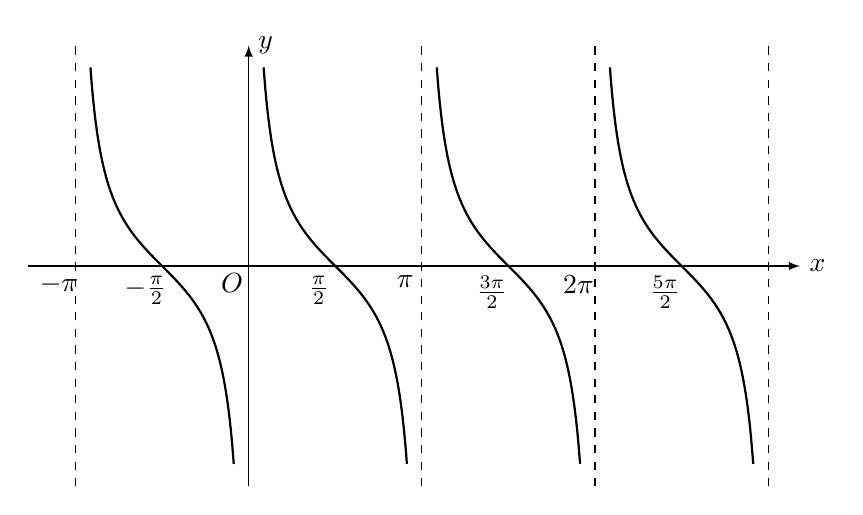
\begin{tikzpicture}[>=latex, scale=.7]
\draw[->] (-4,0)--(10,0)node[right]{$x$};
\draw[->] (0,-4)--(0,4)node[right]{$y$};
\foreach \x/\xtext in {-2/-\pi,-1/-\frac{\pi}{2},1/\frac{\pi}{2},2/\pi,3/\frac{3\pi}{2},4/2\pi,5/\frac{5\pi}{2}}
{
    \node at (\x*.5*pi-.3,0)[below]{$\xtext$};
}

\foreach \x in {-1,1,2,3}
{
    \draw[dashed] (\x*pi,-4)--(\x*pi,4);
}

\node at (-.3,-.3){$O$};

\foreach \y in {-1,1,3,5}
{
    \draw [domain=\y*0.5*pi-1.3 : \y*0.5*pi+1.3, samples=1000, thick] plot(\x, {cot (\x r) });
}

\end{tikzpicture}
